\chapter{Validation Test Cases}
\label{cha:tests}


\section{Introduction}

In order to validate the coupling adapter developed in this work, a set of test cases have been simulated, which are supposed to qualitatively and quantitatively confirm the physically correctness of the implementation.

The validation has been carried out in different steps: the first task (section \ref{sec:dummy}) consisted in validating the MBDyn model that has been used throughout the simulations and verifying that the implementation of the coupling works as expected.

The second step aimed at comparing the results obtained performing an FSI simulation with MBDyn with another structural solver, both in compressible and in incompressible regime (Sections \ref{sec:cx-mbd} and \ref{sec:su2-mbd}).

Then, some results obtained from FSI simulations coupling MBDyn with OpenFOAM, have been compared with some benchmarks present in literature. At first, the problem described in \cite{ramm1998fluid} has been considered (see Section \ref{sec:sq-cyl-bench}): it is composed of a square cylinder with a trailing flap. It is characterized by a mass ratio (see Section \ref{subsec:mass-ratio}) of $1.18\cdot 10^{-3}$, this turned out to be a fundamental parameter fo the convergence of simulations, and has been extensively analyzed in the subsequent sections.

One set of well-known benchmarks in FSI literature are the three Turek-Hron FSI test cases described in \cite{turek2006proposal}. Those cases are characterized by the same domain (a round cylinder with a trailing flap) and the same fluid properties. Changes impact only fluid velocity and structural properties (in particular $\rho,E$).

At first, the so-called FSI2 benchmark (characterized by a mass number of $0.1$) has been considered (Section \ref{sec:FSI2}). This benchmark, together with the previous one, shows the validity of the adapter and its potential use in FSI simulations.

Finally, the FSI3 benchmark has been extensively analyzed (Section \ref{sec:FSI1-FSI3}). It has a mass number of $1$ and, up to now, it hasn't been possible to find a suitable set of coupling parameters that can make this case converge when coupled with MBDyn.

It appears that the added mass effect (see Section \ref{sec:added-mass}), plays a dominant role in the convergence of a FSI problems with MBDyn. For this reason, a sensitivity analysis has been performed on the FSI3 problem setup (Section \ref{sec:FSI3-sensitivity}). In particular, flow velocity, fluid density and solid stiffness have been varied in order to gain some insight about the range of parameters, and adimensional numbers that must be considered to understand how critical a simulation can be.     

Each section starts with a short description of the test case, including the most relevant parameter: e.g. the fluid domain geometry and discretization, structural and coupling parameters. Finally some results are presented, together with the coupling performances.

The meshes for all test cases have generated with the free software \textit{Salome}\footnote{\href{https://www.salome-platform.org/}{salome-platform.org/}}. Files for MBDyn interface points have been generated by a Python script running within the \textit{Salome} environment. The script is part of the software made for this work. 


\section{Dummy fluid solver}
\label{sec:dummy}

The first task implemented to validate the adapter consisted in developing a simple \textit{dummy fluid solver}: i.e. a software component connected to the coupling library preCICE with the simple task to apply forces to user-defined nodes on the structure and read back the displacements of the interface nodes.

This approach allowed first to validate the MBDyn model with the \texttt{external structural mapping} component (see Section \ref{sec:mbd-forces}) and the correct data exchange between preCICE and the adapter. 

The \textit{dummy solver} has been written in Python and it is part of the software package in this work.

A MBDyn cantilever beam model composed of 5 \texttt{beam3} elements (see Section \ref{sec:mbd-beam}) has been written to perform this test, as depicted in Figure \ref{fig:cnt-beams}. This requires a total of 11 \texttt{node} elements to define the structure.

The beam section is uniform and rectangular ($w \times h$) and the physical properties (eg. $\rho, E, \nu$) are constant throughout the beam length. 

\begin{figure}[htbp!]
	    \centering
        \begin{tikzpicture}
            \point{a}{0}{0};
            \point{b}{1.5}{0};
            \point{c}{3}{0};
            \point{d}{4.5}{0};
            \point{e}{6}{0};
            \point{f}{7.5}{0};
            
            \beam{4}{a}{b};
            \beam{4}{b}{c};
            \beam{4}{c}{d};
            \beam{4}{d}{e};
            \beam{4}{e}{f};
            
            \notation{2}{b}{};
            \notation{2}{c}{};
            \notation{2}{d}{};
            \notation{2}{e}{};
            \notation{2}{f}{};
            
            \notation{4}{a}{b}[ $1$ ];
            \notation{4}{b}{c}[ $2$ ];
            \notation{4}{c}{d}[ $3$ ];
            \notation{4}{d}{e}[ $4$ ];
            \notation{4}{e}{f}[ $5$ ];
            
            \support{3}{a}[-90];
            % \load{1}{b}[90][1][.1];
            
            \dimensioning{1}{a}{f}{-1.8}[$L$];
            \dimensioning{1}{a}{b}{-1}[$l$];
            
            \dscaling{3}{0.5};
            \daxis{1}{-1.5 ,0 ,0}[right][above][left];
        \end{tikzpicture}
    	\caption{cantilever made of 5 beam elements}
		\label{fig:cnt-beams}
\end{figure}

The inertia of the structure is provided by 2 \texttt{body} elements (see Section \ref{sec:mbd-body} attached to the second and third nodes of each beam (see Figure \ref{fig:mbdyn-beam-model}). The center of gravity of each body is offset by $-l/4$ in x-direction (where $l$ is the length of the single beam element). Each body has the following inertial properties (see Figure \ref{fig:cnt-mass}): 

\begin{equation}
    m = \rho wh \frac{l}{4} \quad I = \frac{m}{12} \begin{bmatrix} h^2+w^2 & 0 & 0 \\ 0 & \frac{l^2}{16} + w^2 & 0 \\ 0 & 0 & \frac{l^2}{16} + h^2 \end{bmatrix}
    \label{eq:body-inertia}
\end{equation}


\begin{figure}[htbp!]
	    \centering
\begin{tikzpicture}[every edge quotes/.append style={auto, text=blue}]
  \pgfmathsetmacro{\cubex}{4}
  \pgfmathsetmacro{\cubey}{2}
  \pgfmathsetmacro{\cubez}{3}
  \draw [draw=blue, every edge/.append style={draw=blue, densely dashed, opacity=.5}, fill=yellow!10]
    (0,0,0) coordinate (o) -- ++(-\cubex,0,0) coordinate (a) -- ++(0,-\cubey,0) coordinate (b) edge coordinate [pos=1] (g) ++(0,0,-\cubez)  -- ++(\cubex,0,0) coordinate (c) -- cycle
    (o) -- ++(0,0,-\cubez) coordinate (d) -- ++(0,-\cubey,0) coordinate (e) edge (g) -- (c) -- cycle
    (o) -- (a) -- ++(0,0,-\cubez) coordinate (f) edge (g) -- (d) -- cycle;
  \path [every edge/.append style={draw=black, |-|}]
    (b) +(0,-5pt) coordinate (b1) edge ["$l/2$"] (b1 -| c)
    (b) +(-5pt,0) coordinate (b2) edge ["h"] (b2 |- a)
    (c) +(3.5pt,-3.5pt) coordinate (c2) edge ["w"] ([xshift=3.5pt,yshift=-3.5pt]e)
    ;
    \daxis{1} {-8,-1,-1.5} [right][above][left];
    \dpoint{q}{-2.5}{-1}{-1.5};
    \dpoint{r}{0}{-1}{-1.5};
    \dpoint{s}{-\cubex}{-1}{-1.5};
    \dpoint{t}{\cubex}{-1}{-1.5};
    \beam{4}{q}{r};
    \dhinge{1}{q};
    \dhinge{1}{r};
    \dhinge{1}{s};
    \dhinge{1}{t};
    \dnotation{1}{q}{CoG};
    \dnotation{1}{r}{$n_2$};
    \dnotation{1}{s}{$n_1$};
    \dnotation{1}{t}{$n_3$};
    \ddimensioning{xy}{q}{r}{1.5}[ $l/4$ ];
    \ddimensioning{xy}{s}{t}{-2.5}[ $l$ ];
    
\end{tikzpicture}
    	\caption{\texttt{body} element attached to node 2 of the \texttt{beam} element}
		\label{fig:cnt-mass}
\end{figure}


The first node of the structure is clamped (to implement the cantilever constraint), while all other joints are constrained to move in the $x-y$ plane and rotate only around the $x-axis$ so that the structure can move only in the $x-y$ plane.
The interface mesh is represented in Figure \ref{fig:mbdyn-mesh}. Only the connectivity elements belonging to the $x-z$ and $y-z$ plane are represented, but it does not affect the behavior if the structure.


\begin{figure}[htbp!]
	\centering
	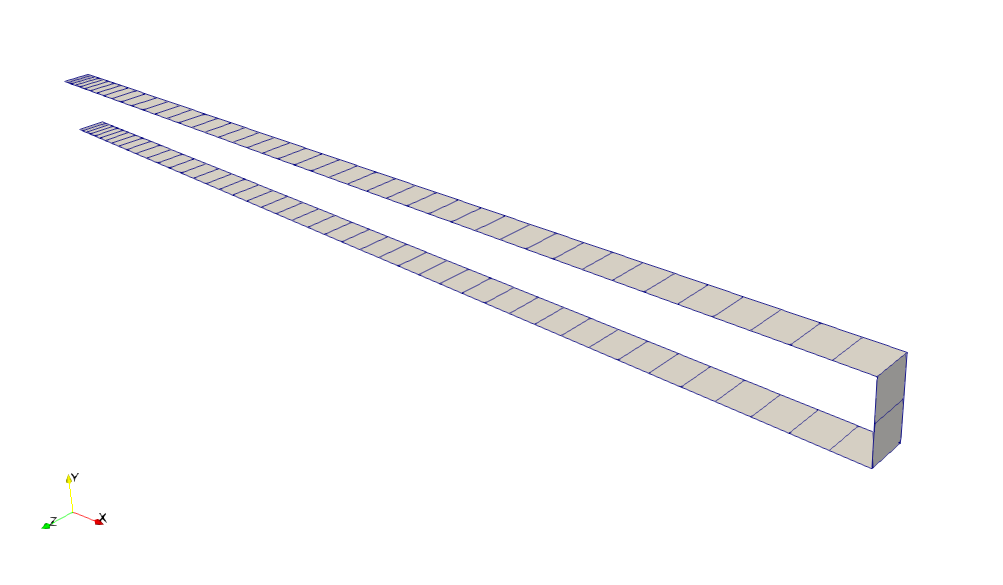
\includegraphics[width=0.7\textwidth]{images/example-mesh}
	\caption{interface points mesh}
	\label{fig:mbdyn-mesh}
\end{figure}

The model has been loaded by a concentrated load on two tip nodes (Figure \ref{fig:cnt-tip}) and with an equivalent distributed load on the nodes belonging to the upper surface (Figure \ref{fig:cnt-distrib}).

\begin{figure}[htbp!]
	%\centering
	    \begin{subfigure}{.8\textwidth}
	    \centering
        \begin{tikzpicture}
            \point{a}{0}{0};
            \point{b}{6}{0};
            \beam{4}{a}{b};
            \support{3}{a}[-90]
            \load{1}{b}[90][1][.1];
        \end{tikzpicture}
    	\caption{cantilever with tip load}
		\label{fig:cnt-tip}
	    \end{subfigure}
	    %\newline
	    \par\bigskip
	    \begin{subfigure}{.8\textwidth}
		\centering
		\begin{tikzpicture}
            \point{a}{0}{0};
            \point{b}{6}{0};
            \beam{4}{a}{b};
            \support{3}{a}[-90]
            \lineload{1}{a}{b}[1][1];%[force interval];
        \end{tikzpicture}
    	\caption{cantilever with distributed load}
		\label{fig:cnt-distrib}
	    \end{subfigure}
	\caption{model and data exchange test-cases}
\end{figure}

The results have been compared the expected theoretical values in terms of tip displacement at steady state and in terms of frequency of the tip movement when the system has been loaded with a step load.

When both the MBDyn model and the data exchanged through the preCICE interface have been validated, the model has been coupled to a CFD solver.





\section{Vertical flap: incompressible regime}
\label{sec:cx-mbd}

The first validation step consisted in comparing the results obtained with MBDyn with the ones given by another structural solver with the same fluid model. 

For this purpose a simple case of a vertical flap immersed in a flow in incompressible regime, has been considered, borrowing an example given in the preCICE website.

\subsection{Fluid domain}

The fluid domain is represented in Figure \ref{fig:ex1-domain}. The inlet is on the left with uniform flow velocity, the outlet is on the right, while all other boundaries are \textit{no-slip} walls.


\begin{figure}[htbp!]
	\centering
	\begin{tikzpicture}
	    \pgfmathsetmacro{\xa}{-0.1}
	    \pgfmathsetmacro{\xb}{0.1}
		\point{a}{-4}{0};
		\point{b}{\xa}{0};
		\point{c}{\xb}{0};
		\point{d}{8}{0};
		\point{e}{\xa}{1};
		\point{f}{\xb}{1};
		\point{g}{-4}{3};
		\point{h}{8}{3};
		
		\point{i}{-3.5}{0.5};
		
		\beam{2}{a}{b};
		\beam{2}{c}{d};
		\beam{2}{a}{g};
		\beam{2}{d}{h};
		\beam{2}{g}{h};
		\beam{4}{b}{e};
		\beam{4}{e}{f};
		\beam{4}{f}{c};
		
		\dimensioning{1}{g}{h}{3.5}[$20m$];
		\dimensioning{1}{a}{b}{-0.6}[$4m$];
		\dimensioning{2}{d}{h}{8.5}[$4m$];
		
		\dimensioning{1}{e}{f}{1.25}[$0.1m$];
		\dimensioning{2}{c}{f}{0.8}[$1m$];
		
		\lineload{1}{a}{g};
		
		\load{1}{i}[180][1][-1];
		\load{1}{i}[-90][1][-1];
		\notation{1}{-2.5,0.25}{x};
		\notation{1}{-3.75,1.5}{z};
		%\dscaling{3}{0.4};
		%\daxis{1}{1.5 ,0 ,0}[right]][above];
	\end{tikzpicture}
	\caption{vertical flap: fluid domain}
	\label{fig:ex1-domain}
\end{figure}


The fluid domain is discretized in an structured hexaedral mesh as depicted in Figure \ref{fig:ex1-mesh}. The main fluid and mesh values are given in Table \ref{table:ex1-fluid} and \ref{table:ex1-mesh}. 

\begin{figure}[htbp!]
	\centering
	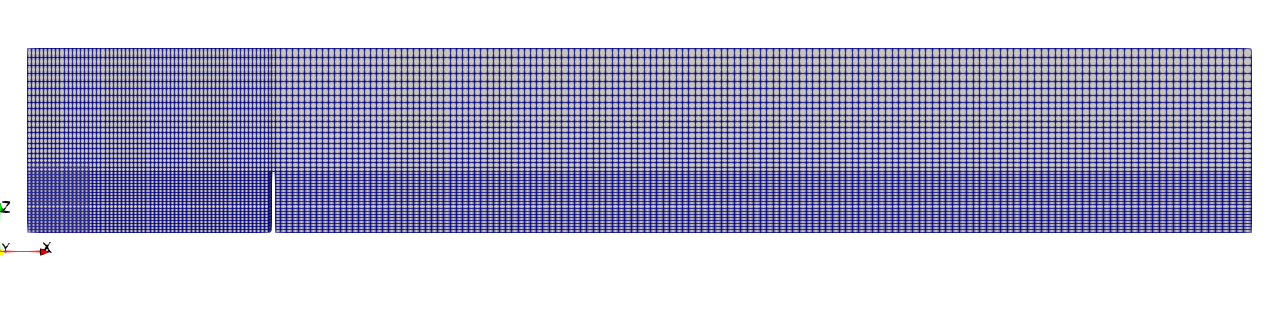
\includegraphics[width=0.9\textwidth]{images/ex1-mesh1}
	\caption{vertical flap: fluid mesh}
	\label{fig:ex1-mesh}
\end{figure}


\begin{table}[!htb]
	\begin{center}
		\begin{tabular}{ l c l | c } 
			parameter & & & value  \\ 
			\hline
			fluid density  & $\rho$ & \si{kg.m^{-3}} & 1   \\
			kinematic viscosity & $\nu$& \si{m^2.s^{-1}} & $10^{-3}$  \\
%			Reynolds length & $l_{Re}$ & $0.1$ & \si{m} \\
%			Reynolds number & Re & $\approx 1000$ & \\
			flow velocity & $\vec{v}$& \si{m.s^{-1}} & 10 \\
			flow type & & & laminar \\
		\end{tabular}
	\end{center}
	\caption{Vertical flap: fluid properties}
	\label{table:ex1-fluid}
\end{table}



\begin{table}[!htb]
	\begin{center}
		\begin{tabular}{ l c | c } 
			parameter & & value   \\ 
			\hline
			number of mesh points  & $n_{dof}$ & 17344     \\
			number of cells & $n_c$ & 8400  \\
			number of interface cells  & $n_{int}$ & 42  \\			
		\end{tabular}
	\end{center}
	\caption{Vertical flap: mesh properties}
	\label{table:ex1-mesh}
\end{table}



\subsection{Simulation and Coupling parameters}

The coupling between the fluid solver and the structural solver is the same for the MBDyn and the CalculiX simulation. The main data are given in Table \ref{table:ex1-coupling}:


\begin{table}[!htb]
	\begin{center}
		\begin{tabular}{ l c  l| c } 
			parameter & & & value   \\ 
			\hline
			simulation time  & $t$& \si{s} & 5      \\
			step size & $\Delta t$ & \si{s} & $10^{-2}$   \\
			\hline
			coupling scheme & & & serial implicit  $S\rightarrow F$  \\
			coupling algorithm & & &  IQN-ILS  \\
			displacement rel. convergence limit & & & $10^{-4}$ \\
			force rel. convergence limit &&  & $10^{-3}$  \\
      		interface mesh mapping & & & RBF  \\
			
		\end{tabular}
	\end{center}
	\caption{Vertical flap: coupling parameters}
	\label{table:ex1-coupling}
\end{table}





\subsection{Structural Solver: CalculiX}

The structural model built in CalculiX is composed of 40 \textbf{C3D8}\footnote{general purpose linear brick element with 8 nodes} as represented in Figure \ref{fig:cx-mesh}. 

\begin{figure}[htbp!]
	\centering
	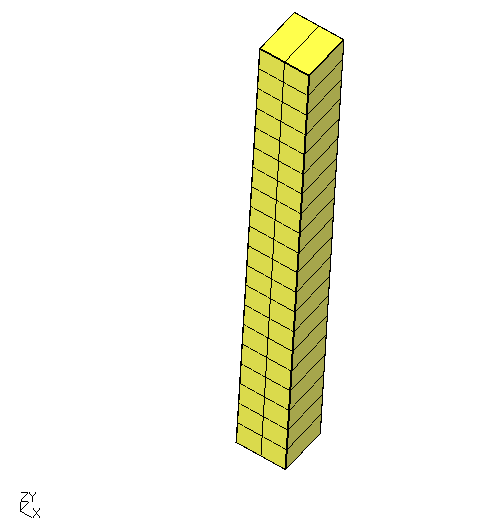
\includegraphics[width=0.6\textwidth]{images/cx1}
	\caption{vertical flap: CalculiX mesh}
	\label{fig:cx-mesh}
\end{figure}

The properties of the solid are reported in Table \ref{table:ex1-solid}.

\begin{table}[!htb]
	\begin{center}
		\begin{tabular}{ l c  l | c } 
			parameter & & value &    \\ 
			\hline
			solid density  & $\rho$ & \si{kg.m^{-3}} & 3000    \\
			Elastic modulus  & E & \si{Pa} & $4\cdot 10^6$    \\
			Poisson coefficient & $\nu$ & & $0.3$  \\
			%			Reynolds length & $l_{Re}$ & $0.1$ & \si{m} \\
			%			Reynolds number & Re & $\approx 1000$ & \\
		\end{tabular}
	\end{center}
	\caption{Vertical flap: solid properties}
	\label{table:ex1-solid}
\end{table}

 
\subsection{Implementation with MBDyn}


The MBDyn model uses the same solid properties of Table \ref{table:ex1-solid} and is composed of 10 \texttt{beam3} elements. Apart from the different orientation, the setup is the same as the one briefly described in Section \ref{sec:dummy}. The only relevant parameter that can be explicitly set up in MBDyn in comparison to CalculiX, consists in the structural damping of the beam elements (see Section \ref{sec:mbd-beam}), which is set to be proportional to stiffness matrix of the element with a coefficient of $2\cdot10^{-3}$.

The interface mesh is divided into 20 faces for the front and back surfaces of the flap. The upper surface is divided into 2, so that the interface is identical to the one obtained in CalculiX. 



\subsection{Results}

The problem considered is characterized by the adimensional parameters given in Table \ref{table:ex1-adim} and its solution is represented in Figure \ref{fig:vf_sol}.


\begin{table}[!htb]
	\begin{center}
		\begin{tabular}{ l c | r } 
			parameter & & value   \\ 
			\hline
			mass number  & $M$ & $3.3\cdot 10^{-4}$     \\
			reduced velocity & $U_R$ & $9.13\cdot 10^{-5}$  \\
			Cauchy number  & $C_Y$ & $2.5\cdot 10^{-5}$  \\			
		\end{tabular}
	\end{center}
	\caption{Vertical flap: adimensional numbers}
	\label{table:ex1-adim}
\end{table}

\begin{figure}[htbp!]
	\centering
	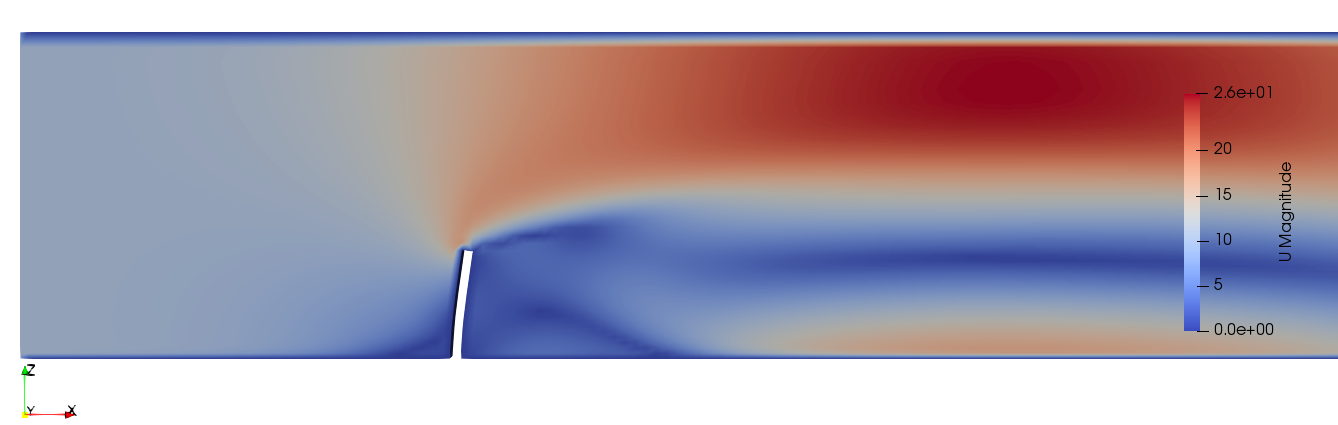
\includegraphics[width=0.9\textwidth]{images/vert_flap/vert_flap1.png}
	\caption{vertical flap: velocity field}
	\label{fig:vf_sol}
\end{figure}


The solutions between CalculiX and MBDyn are first compared in terms of resultants applied to the structure during the simulation (Figures \ref{fig:vf_force} and \ref{fig:vf_moment}), then the tip displacement in $x$ direction is considered in Figure \ref{fig:vf_displacement}. The forces and moments applied to the structure in the two cases are very close. 
The tip displacement shows that both structures exhibit the same damping and the oscillating frequency is very close: CalculiX shows a slightly higher frequency and a more visible second order frequency. The MBDyn structure looks a little more flexible: after 50 seconds of simulation tends to $58mm$ of tip displacement in $x$ direction, while the same structure in CalculiX tends to $53mm$ of displacement. 

\begin{figure}[htbp!]
	\centering
	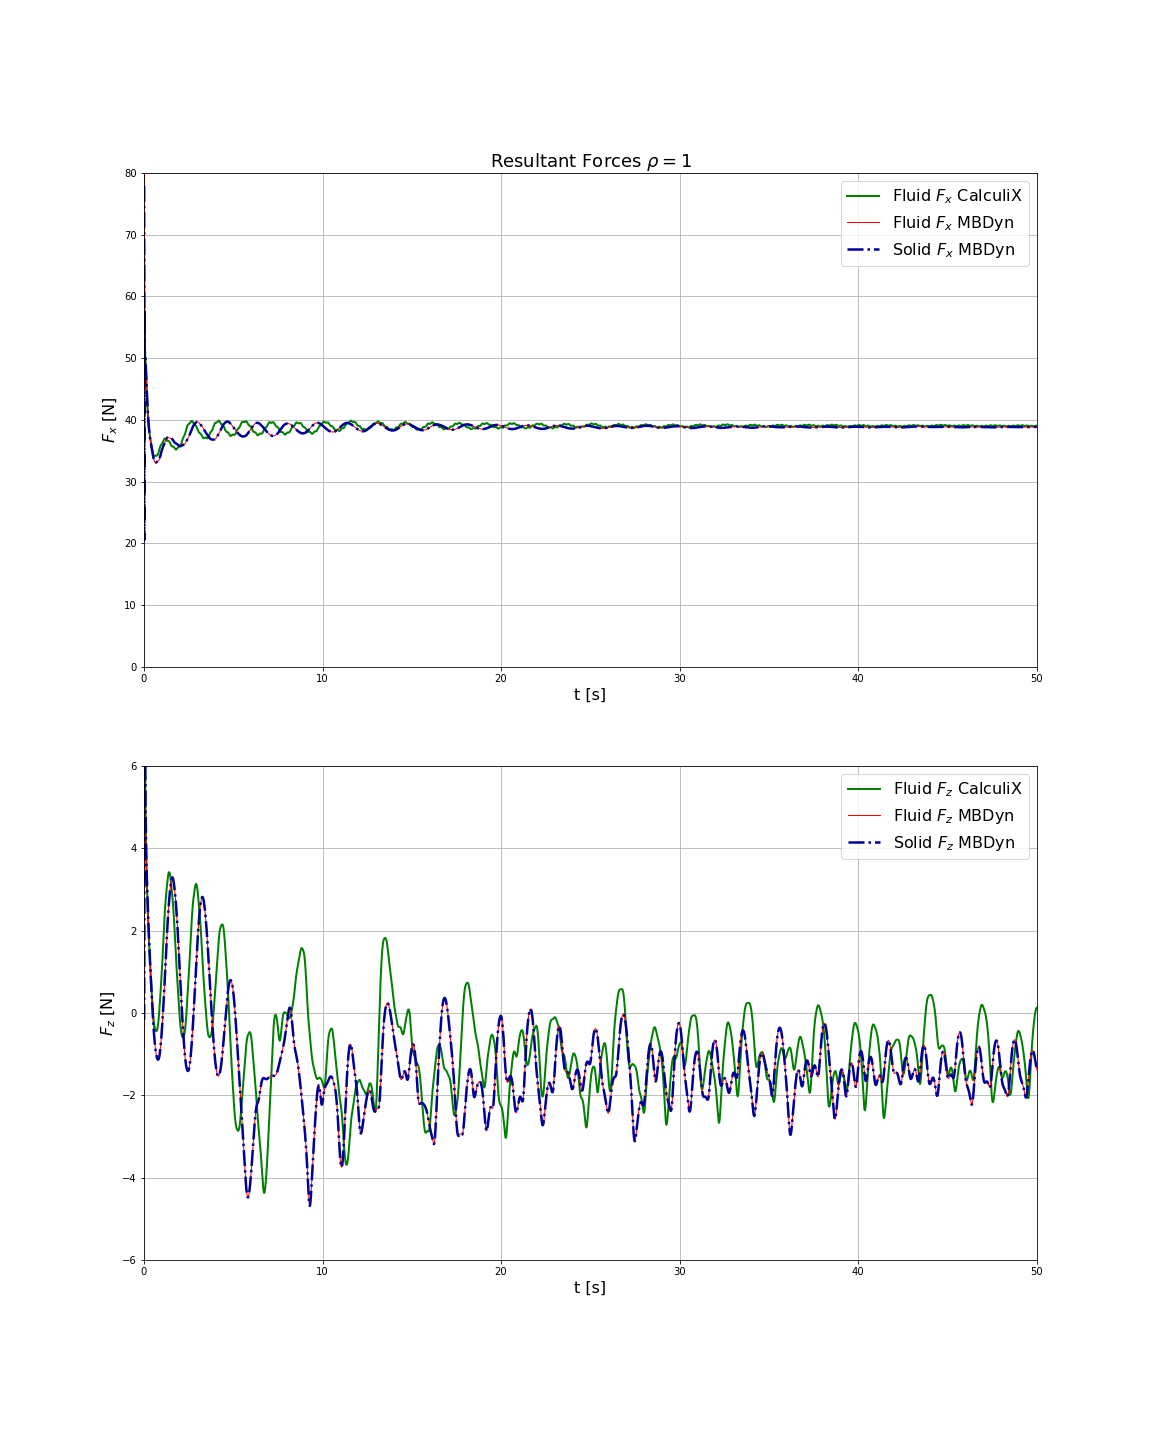
\includegraphics[width=0.9\textwidth]{images/vert_flap/forces_rho1.png}
	\caption{vertical flap: resultant forces}
	\label{fig:vf_force}
\end{figure}

\begin{figure}[htbp!]
	\centering
	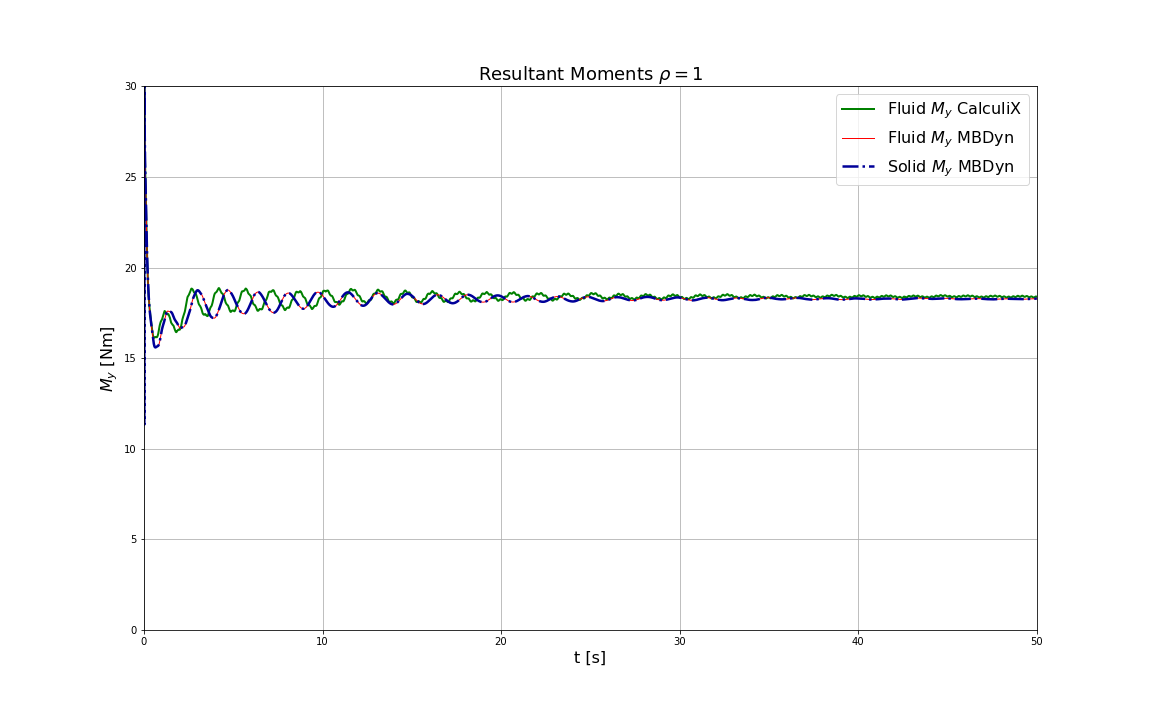
\includegraphics[width=0.9\textwidth]{images/vert_flap/moments_rho1.png}
	\caption{vertical flap: moment applied at root}
	\label{fig:vf_moment}
\end{figure}



\begin{figure}[htbp!]
	\centering
	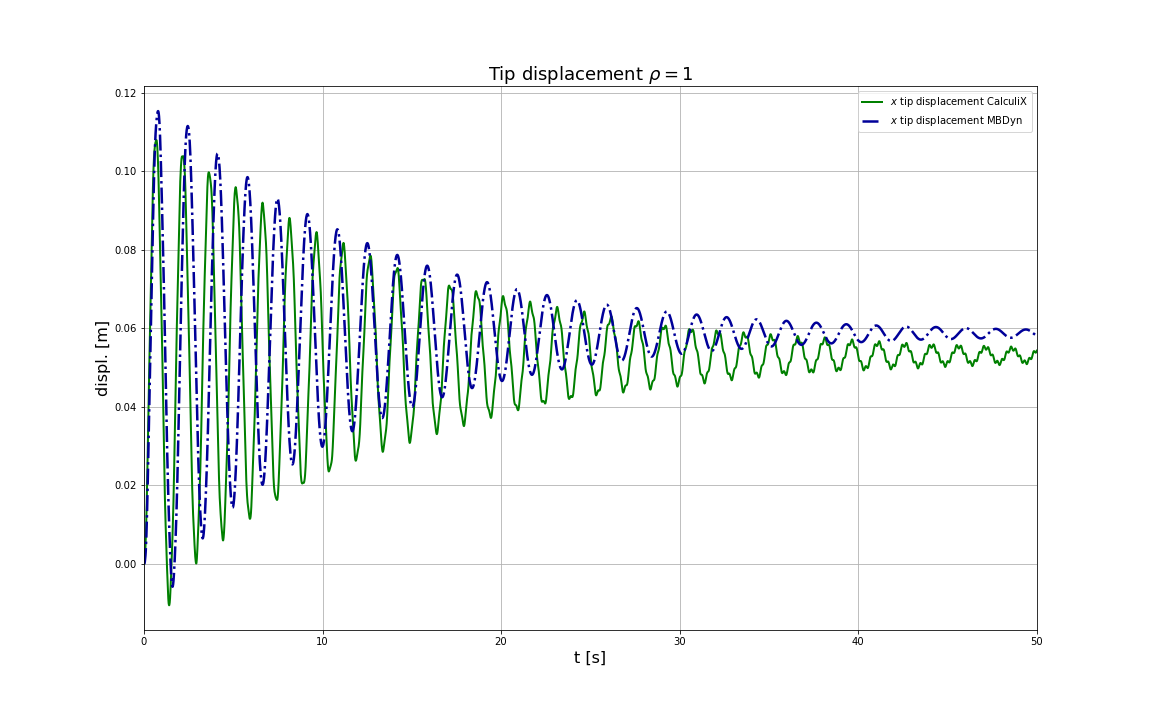
\includegraphics[width=0.9\textwidth]{images/vert_flap/disp_rho1.png}
	\caption{vertical flap: tip displacement x direction}
	\label{fig:vf_displacement}
\end{figure}


As to convergence and number of iterations between the two solvers, Figure \ref{fig:vf_cx_iter} and \ref{fig:vf_mbd_iter} show that, in general, MBdyn and CalculiX require 2 iterations to converge. This can be explained by the small mass number of this case. At some iterations MBDyn requires more iterations: this is due to the fact, for some reasons due to the coupling not completely understood at the moment, a force unbalance arises in the y-direction (out of the plane of the model) which produces a moment around x-axis. This moment is absorbed by the rotation constraints at the nodes and it does not affect the behavior of the resultant in x and z directions. 

\begin{figure}[htbp!]
	\centering
	\begin{subfigure}{0.8\textwidth}
	\centering
	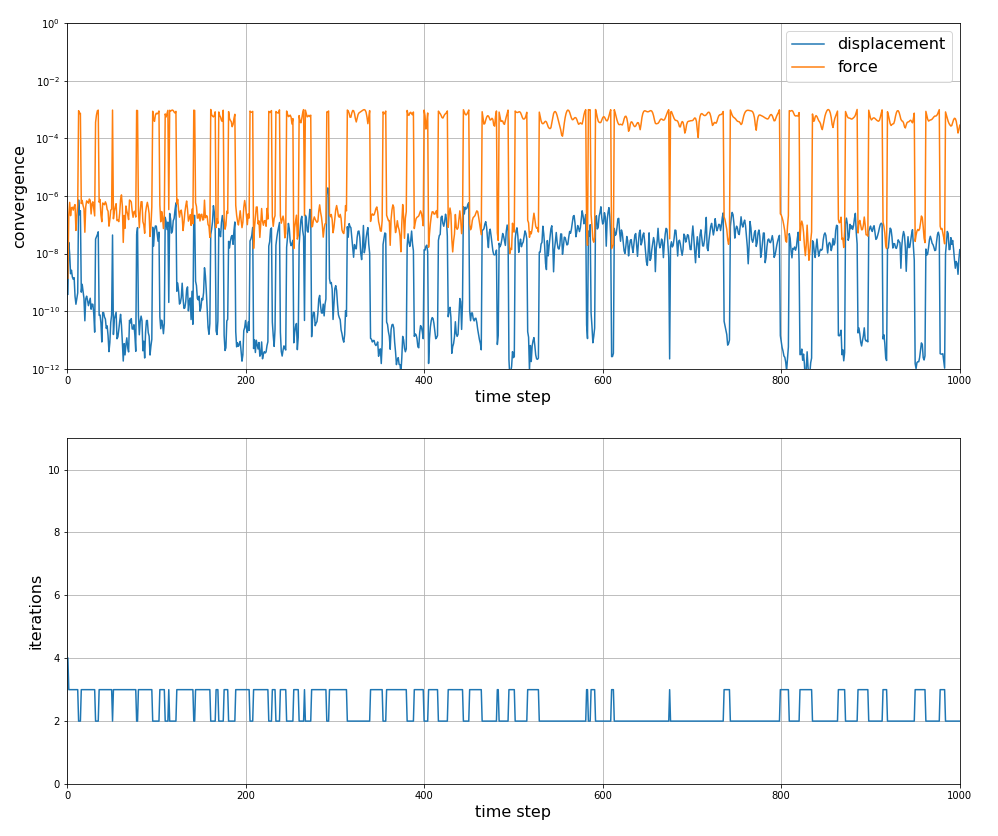
\includegraphics[width=\textwidth, trim=0 0 0 20, clip]{images/vert_flap/CX_iterations_rho1.png}
	\caption{CalculiX}
	\label{fig:vf_cx_iter}
	\end{subfigure}
	\begin{subfigure}{0.9\textwidth}
	\centering
	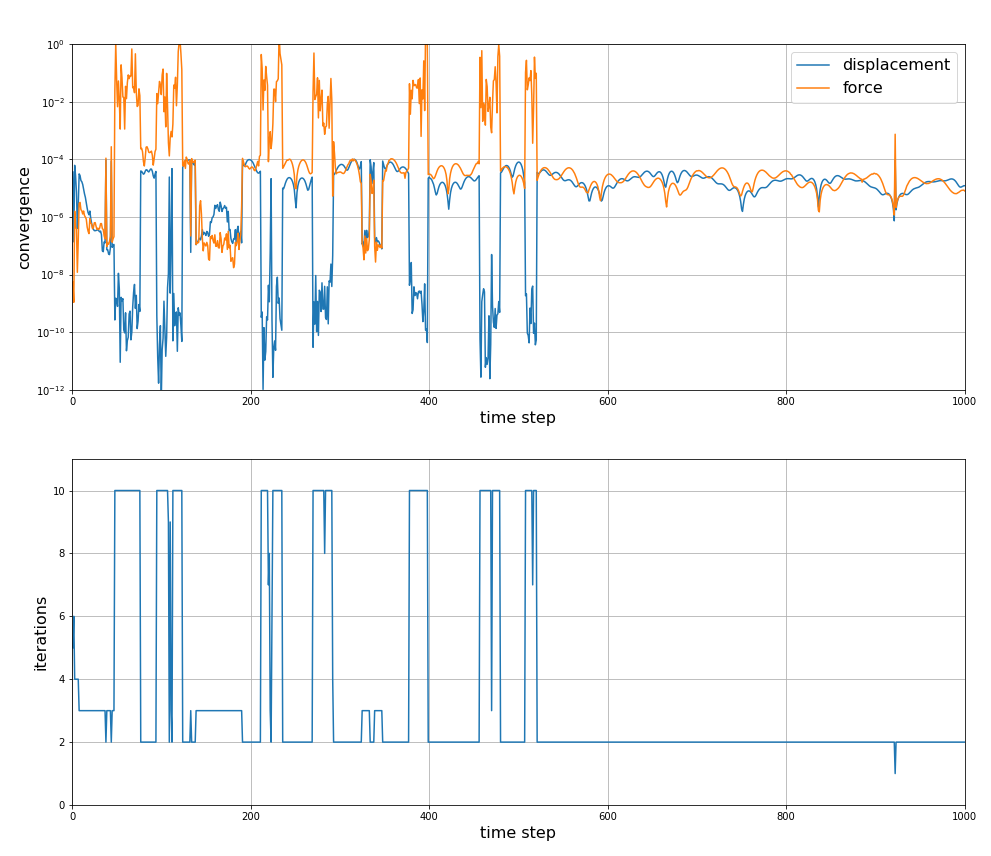
\includegraphics[width=\textwidth, trim=0 0 0 20, clip]{images/vert_flap/MBD_iterations_rho1.png}
	\caption{MBDyn}
	\label{fig:vf_mbd_iter}
	\end{subfigure}
	\caption{vertical flap: convergence and iterations}
	\label{fig:vf_iter}
\end{figure}


Finally, MBDyn allows to analyze the internal forces of each beam, as represented in Figure \ref{fig:vf_mbd_internal}.

\begin{figure}[htbp!]
	\centering
	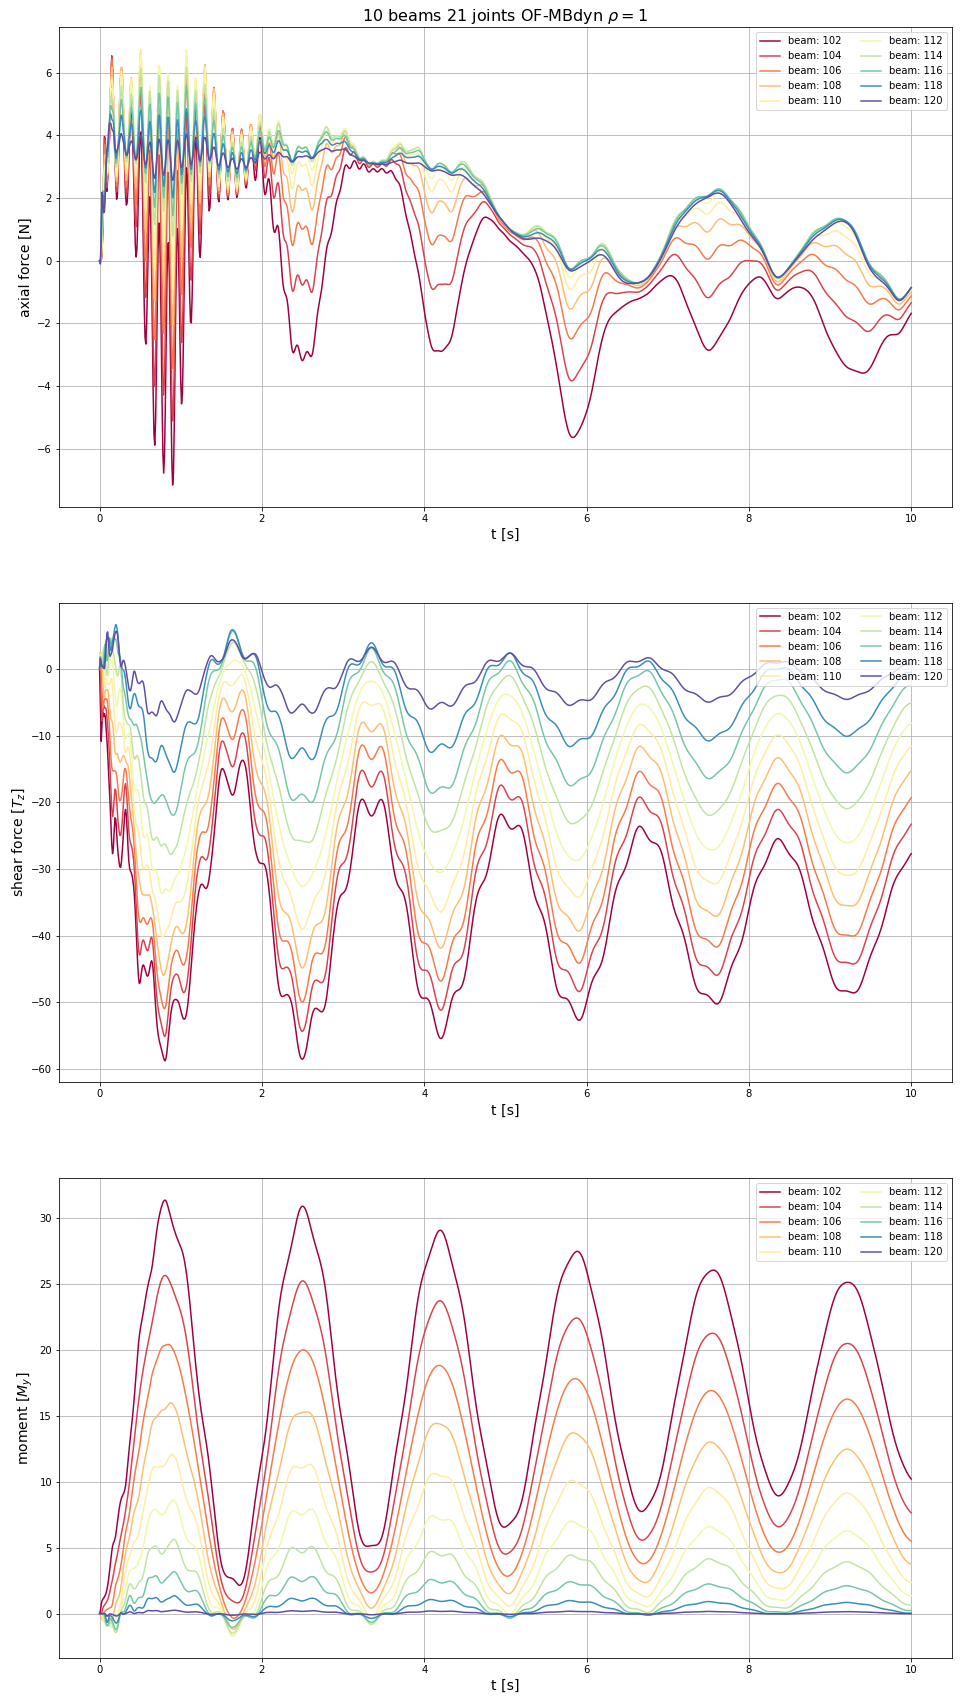
\includegraphics[width=0.82\textwidth]{images/vert_flap/OF-MBDyn_rho1_act.png}
	\caption{vertical flap: MBDyn convergence and iterations}
	\label{fig:vf_mbd_internal}
\end{figure}


\newpage

\section{Vertical flap: compressible regime}
\label{sec:su2-mbd}

A model similar to the one described in the previous section has been used to test the coupling capabilities of the adapter with a different fluid solver: SU2\footnote{\href{https://su2code.github.io/}{su2code.github.io}}. The coupling adapter between SU2 and preCICE allows to build FSI simulations in compressible regime. Besides, SU2 allows to define strictly bidimensional domains, while OpenFOAM and MBDyn are strictly tridimensional. Bidimensionality is enforced in OenFOAM using \textit{empty} boundary conditions, while in MBDyn is enforced through constraints on nodes.
For those reasons a similar model has been built. 


\subsection{Fluid domain}

The fluid domain is represented in Figure \ref{fig:comp-domain}. The inlet is on the left with uniform flow velocity, the outlet is on the right, while all other boundaries are \textit{slip} walls.


\begin{figure}[htbp!]
	\centering
	\begin{tikzpicture}
	    \pgfmathsetmacro{\xa}{-1.1}
	    \pgfmathsetmacro{\xb}{-1}
		\point{a}{-4}{0};
		\point{b}{\xa}{0};
		\point{c}{\xb}{0};
		\point{d}{8}{0};
		\point{e}{\xa}{1};
		\point{f}{\xb}{1};
		\point{g}{-4}{3};
		\point{h}{8}{3};
		
		\point{i}{-3.5}{0.5};
		
		\beam{2}{a}{b};
		\beam{2}{c}{d};
		\beam{2}{a}{g};
		\beam{2}{d}{h};
		\beam{2}{g}{h};
		\beam{4}{b}{e};
		\beam{4}{e}{f};
		\beam{4}{f}{c};
		
		\dimensioning{1}{g}{h}{3.5}[$4.2m$];
		\dimensioning{1}{a}{b}{-0.6}[$1.2m$];
		\dimensioning{2}{d}{h}{8.5}[$1.2m$];
		
		\dimensioning{1}{e}{f}{1.25}[$0.002m$];
		\dimensioning{2}{c}{f}{-0.2}[$0.4m$];
		
		\lineload{1}{a}{g};
		
		\load{1}{i}[180][1][-1];
		\load{1}{i}[-90][1][-1];
		\notation{1}{-2.5,0.25}{x};
		\notation{1}{-3.75,1.5}{y};
		%\dscaling{3}{0.4};
		%\daxis{1}{1.5 ,0 ,0}[right]][above];
	\end{tikzpicture}
	\caption{vertical flap (compressible): fluid domain}
	\label{fig:comp-domain}
\end{figure}


The fluid domain is discretized in an unstructured triangular mesh as depicted in Figure \ref{fig:comp-mesh}. The main fluid and mesh values are given in Table \ref{table:comp-fluid} and \ref{table:comp-mesh}. 

\begin{figure}[htbp!]
	\centering
	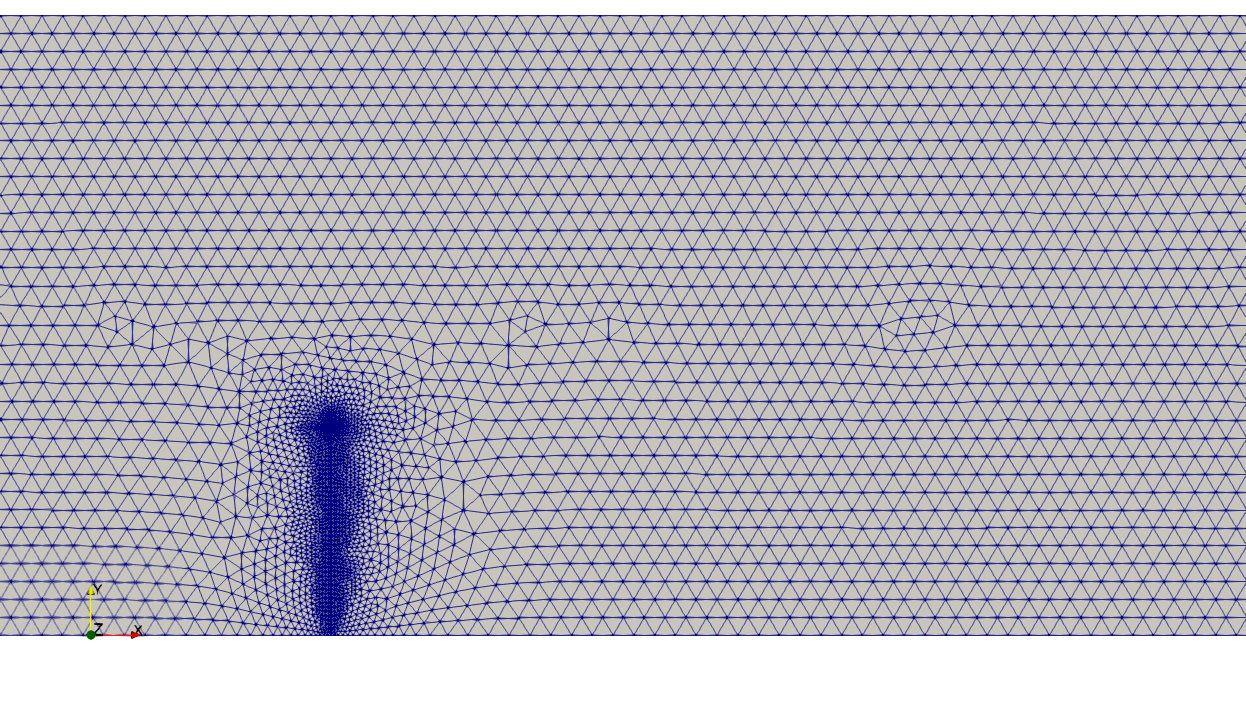
\includegraphics[width=0.9\textwidth, trim=0 100 0 100,clip]{images/comp_flap/mesh.png}
	\caption{vertical flap (compressible): fluid mesh}
	\label{fig:comp-mesh}
\end{figure}


\begin{table}[!htb]
	\begin{center}
		\begin{tabular}{ l c l | c } 
			parameter & & & value  \\ 
			\hline
			fluid properties  &  &  & standard air   \\
			outlet pressure & $p$& \si{Pa} & $101300$  \\
			inlet temperature & $T$ & \si{K} & 288  \\
%			Reynolds number & Re & $\approx 1000$ & \\
			inlet Mach number &  Ma &  & 0.1 \\
			flow type & & & euler \\
		\end{tabular}
	\end{center}
	\caption{Vertical flap (compressible): fluid properties}
	\label{table:comp-fluid}
\end{table}



\begin{table}[!htb]
	\begin{center}
		\begin{tabular}{ l c | c } 
			parameter & & value   \\ 
			\hline
			number of mesh points  & $n_{dof}$ & 5580     \\
			number of cells & $n_c$ & 10709  \\
			number of interface points  & $n_{int}$ & 162  \\			
		\end{tabular}
	\end{center}
	\caption{Vertical flap (compressible): mesh properties}
	\label{table:comp-mesh}
\end{table}


\subsection{MBDyn model}


The MBDyn model uses solid properties defined in Table \ref{table:comp-solid} and is composed of 5 \texttt{beam3} elements. 

\begin{table}[!htb]
	\begin{center}
		\begin{tabular}{ l c  l | c } 
			parameter & & & value   \\ 
			\hline
			solid density  & $\rho$ & \si{kg.m^{-3}} & 1000    \\
			Elastic modulus  & E & \si{Pa} & $ 5.6 \cdot 10^9$    \\
			Poisson coefficient & $\nu$ & & $0.4$  \\
			structural damping & & & $1 \cdot 10^{-3}$ \\
			%			Reynolds length & $l_{Re}$ & $0.1$ & \si{m} \\
			%			Reynolds number & Re & $\approx 1000$ & \\
		\end{tabular}
	\end{center}
	\caption{Vertical flap: solid properties}
	\label{table:comp-solid}
\end{table}

\subsection{Coupling parameters}

The main data concerning the coupling between MBDyn and SU2 are given in Table \ref{table:comp-coupling}:

\begin{table}[!htb]
	\begin{center}
		\begin{tabular}{ l c  l| c } 
			parameter & & & value   \\ 
			\hline
			simulation time  & $t$& \si{s} & 1      \\
			step size & $\Delta t$ & \si{s} & $10^{-3}$   \\
			\hline
			coupling scheme & & & serial implicit $S\rightarrow F$  \\
			coupling algorithm & & &  IQN-ILS  \\
			displacement rel. convergence limit & & & $10^{-5}$ \\
			force rel. convergence limit &&  & $10^{-3}$  \\
      		interface mesh mapping & & & RBF  \\
			
		\end{tabular}
	\end{center}
	\caption{Vertical flap (compressible): coupling parameters}
	\label{table:comp-coupling}
\end{table}


\subsection{results}

The problem considered is characterized by the adimensional parameters given in Table \ref{table:comp-adim}: in particular the mass number remains in the order of $\mathcal{O} \left(10^{-3}\right)$. A sketch of the flow solution is represented in Figure \ref{fig:comp_sol}.

\begin{table}[!htb]
	\begin{center}
		\begin{tabular}{ l c | r } 
			parameter & & value   \\ 
			\hline
			mass number  & $M$ & $ \approx 1.2\cdot 10^{-3}$     \\
			reduced velocity & $U_R$ & $ \approx 1.44\cdot 10^{-5}$  \\
			Cauchy number  & $C_Y$ & $  \approx 2.53 \cdot 10^{-7}$  \\			
		\end{tabular}
	\end{center}
	\caption{Vertical flap (compressible): adimensional numbers}
	\label{table:comp-adim}
\end{table}

\begin{figure}[htbp!]
	\centering
	\begin{subfigure}{0.9\textwidth}
	\centering
	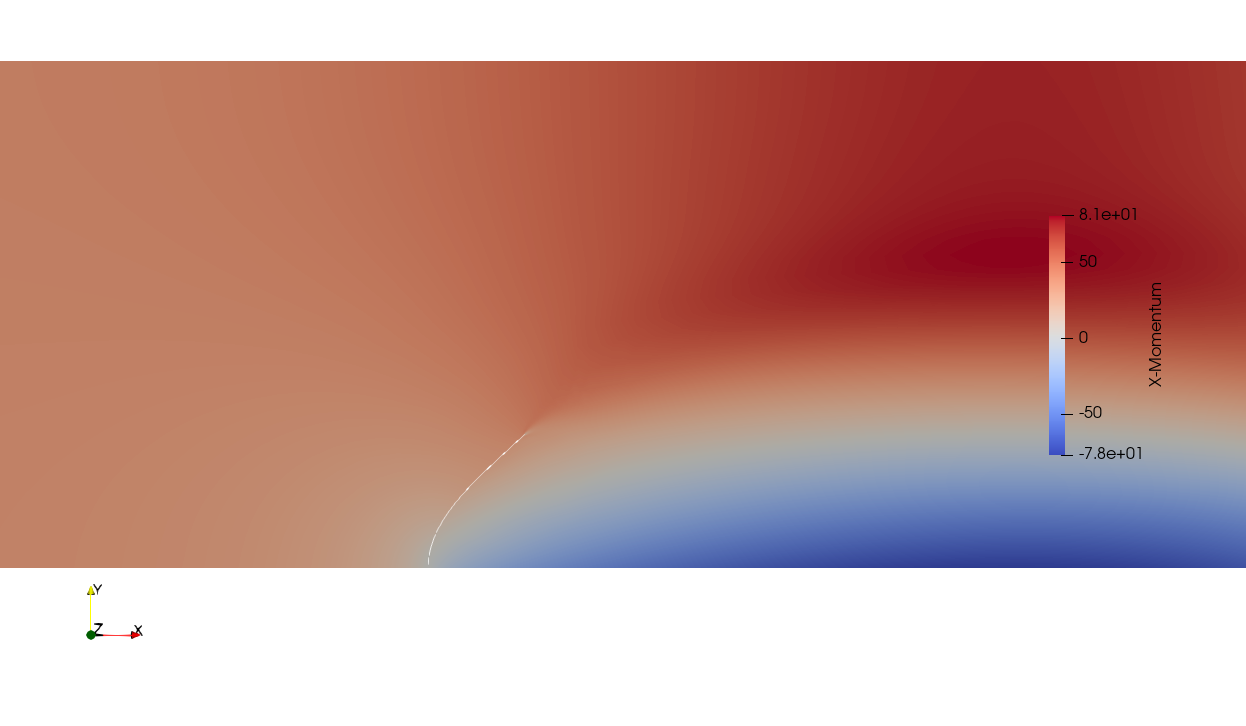
\includegraphics[width=\textwidth, trim=0 150 0 150, clip]{images/comp_flap/x-mom.png}
	\caption{vertical flap (compressible): x-momentum}
	\end{subfigure}
	\begin{subfigure}{\textwidth}
	\centering
	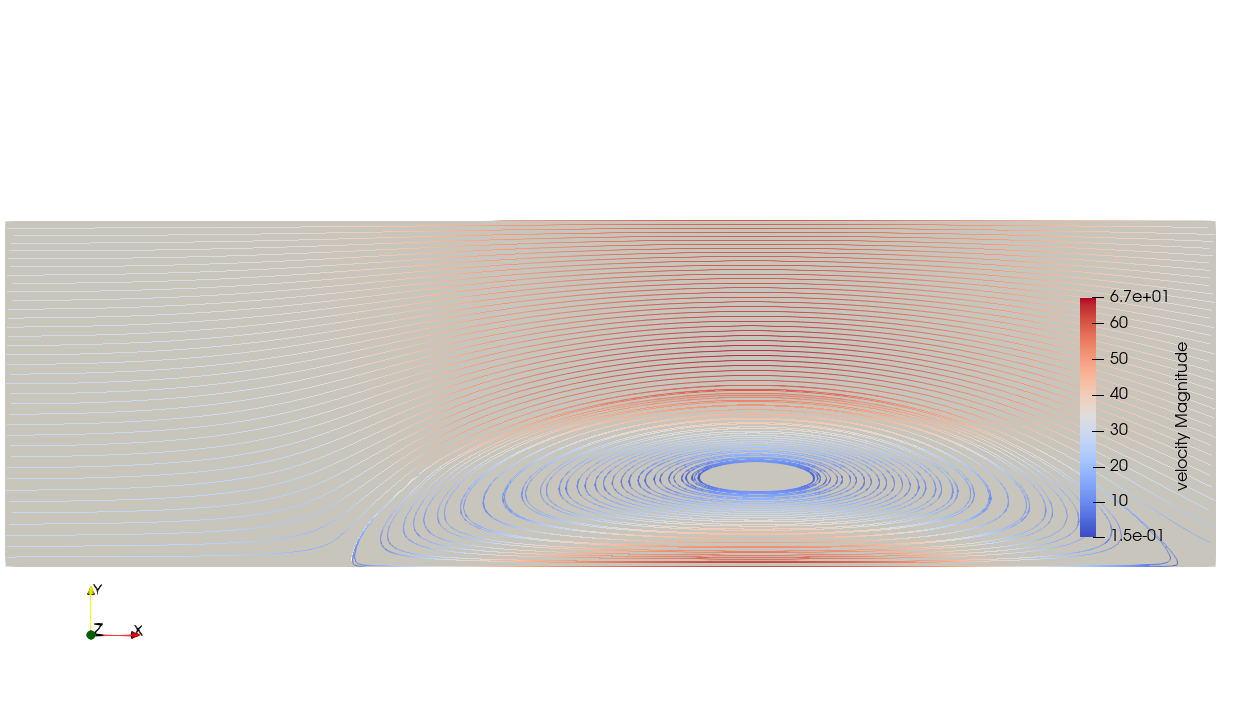
\includegraphics[width=0.95\textwidth, trim=0 150 0 150, clip]{images/comp_flap/vel-stream.png}
	\caption{vertical flap (compressible): streamlines}
	\end{subfigure}
	\caption{vertical flap (compressible): flow solution}
	\label{fig:comp_sol}
\end{figure}


The combination of parameters considered in this test case aimed at considering a very thin flexible element surrounded by a low-Mach flow, so that large displacements are involved. The structure reaches a steady deformed shape after around 1 second as shown in Figure  \ref{fig:comp_displacement}, concerning tip displacement. 

The fluid flow has been initialized with a steady solution obtained considering a rigid structure, then the FSI problem has been simulated applying the the aerodynamic load to the flap progressively: a linear ramp starting at $1\%$ of the load with a duration of 0.2 seconds (see Section \ref{sec:mbdyn-adapter-input} for the adapter input parameters).

Resultant forces $(R_x, R_y)$ and moment $(M_z)$ computed at the root of the flap are shown in Figure \ref{fig:comp_force}.

\begin{figure}[htbp!]
	\centering
	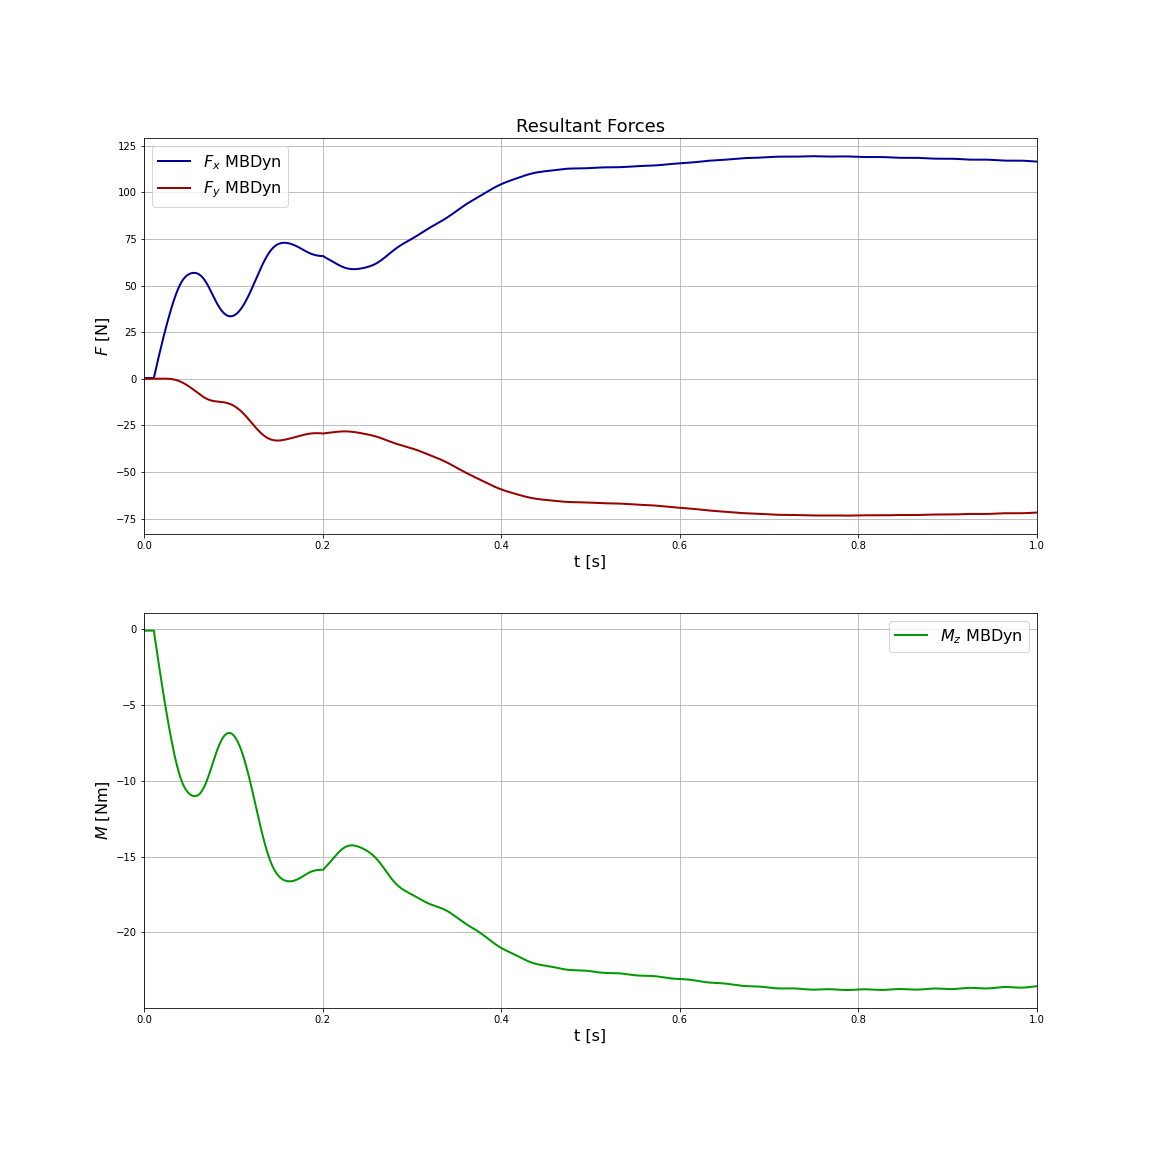
\includegraphics[width=0.9\textwidth, trim=0 100 0 100, clip]{images/comp_flap/forces_comp.png}
	\caption{vertical flap (compressible): resultant forces}
	\label{fig:comp_force}
\end{figure}



\begin{figure}[htbp!]
	\centering
	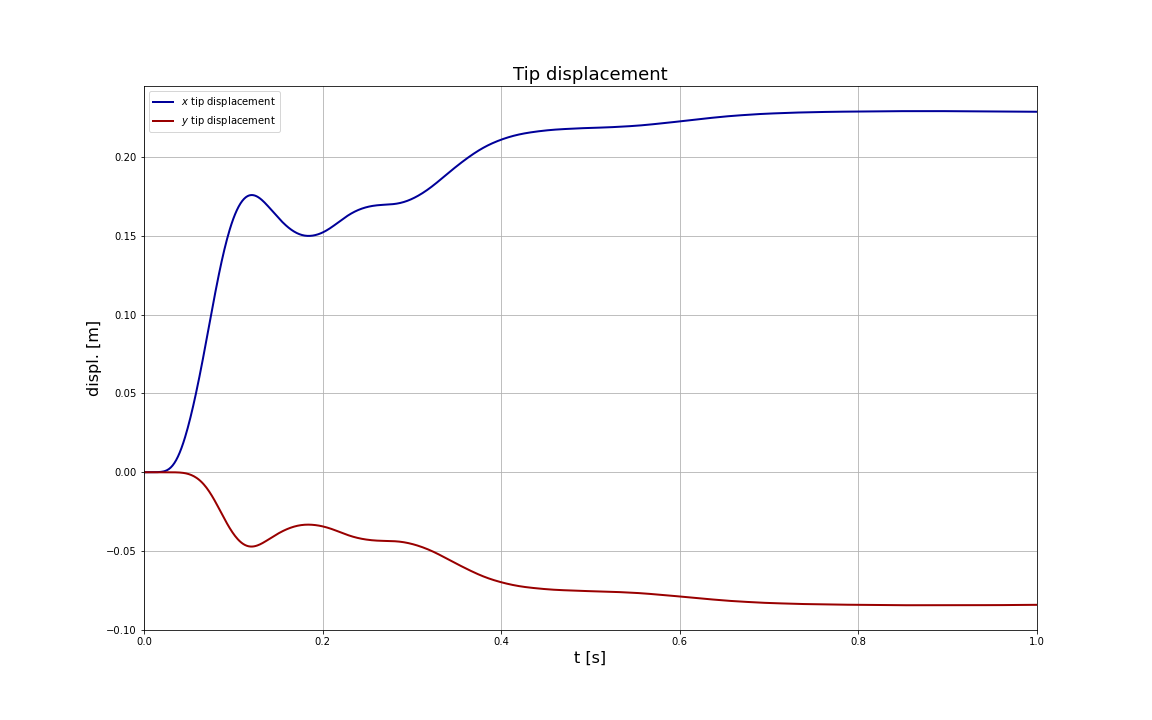
\includegraphics[width=0.9\textwidth, trim=0 50 0 50, clip]{images/comp_flap/disp_comp.png}
	\caption{vertical flap (compressible): tip displacement}
	\label{fig:comp_displacement}
\end{figure}


Each time step of the problem converges quite rapidly, requiring 5 iterations in most cases. This outcome agrees with the fact that a low mass number and a high fluid velocity make the problem loosely coupled (see section \ref{sec:strong-coupling} for some details). Nevertheless an explicit simulation diverges immediately.  


\begin{figure}[htbp!]
	\centering
	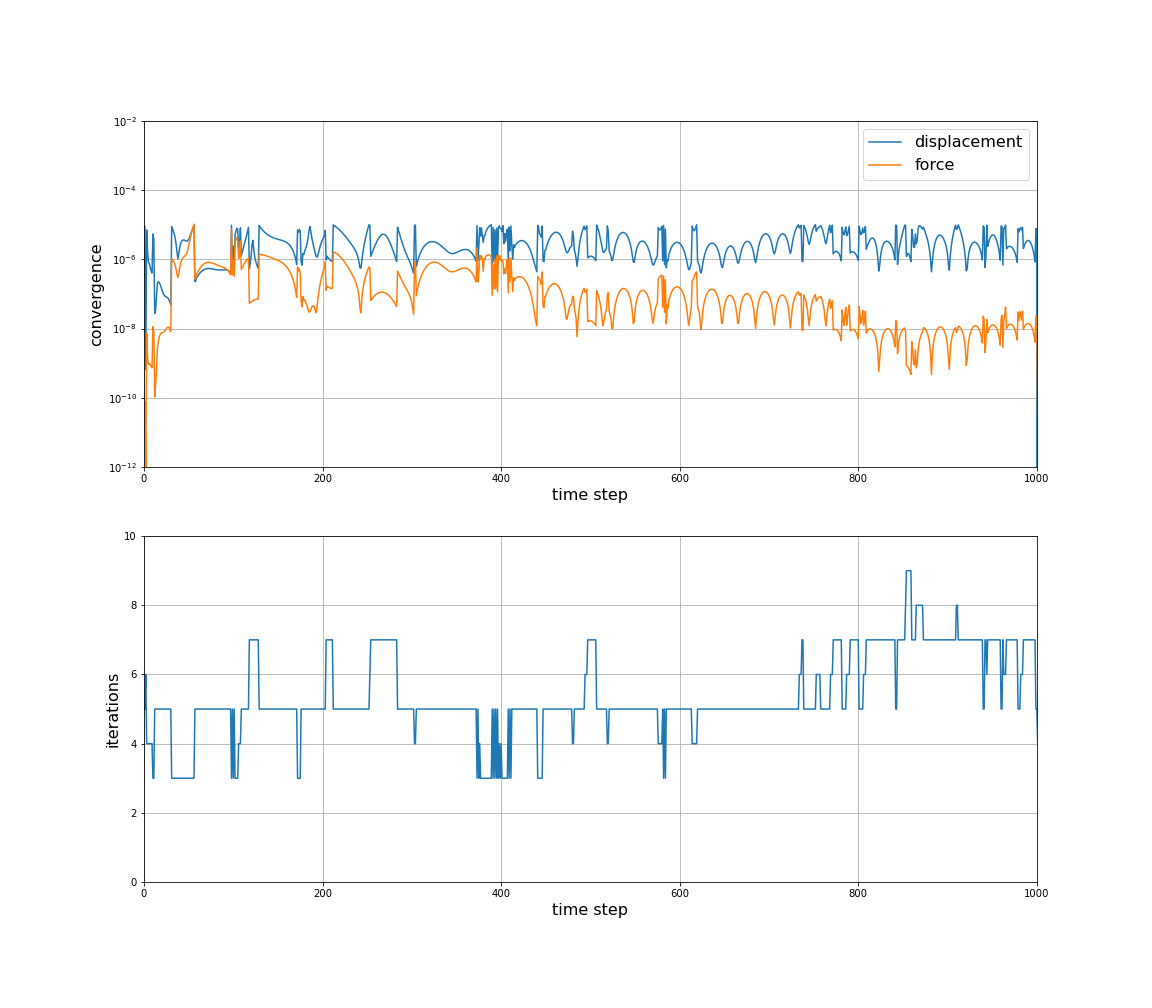
\includegraphics[width=0.95\textwidth, trim=0 80 0 100, clip]{images/comp_flap/MBD_iterations_comp.png}
	\caption{vertical flap (compressible): convergence and iterations}
	\label{fig:comp_mbd_iter}
\end{figure}

Axial, shear and bending moment in each of the MBDyn elements are plotted in Figure \ref{fig:comp_mbd_internal}.

\begin{figure}[htbp!]
	\centering
	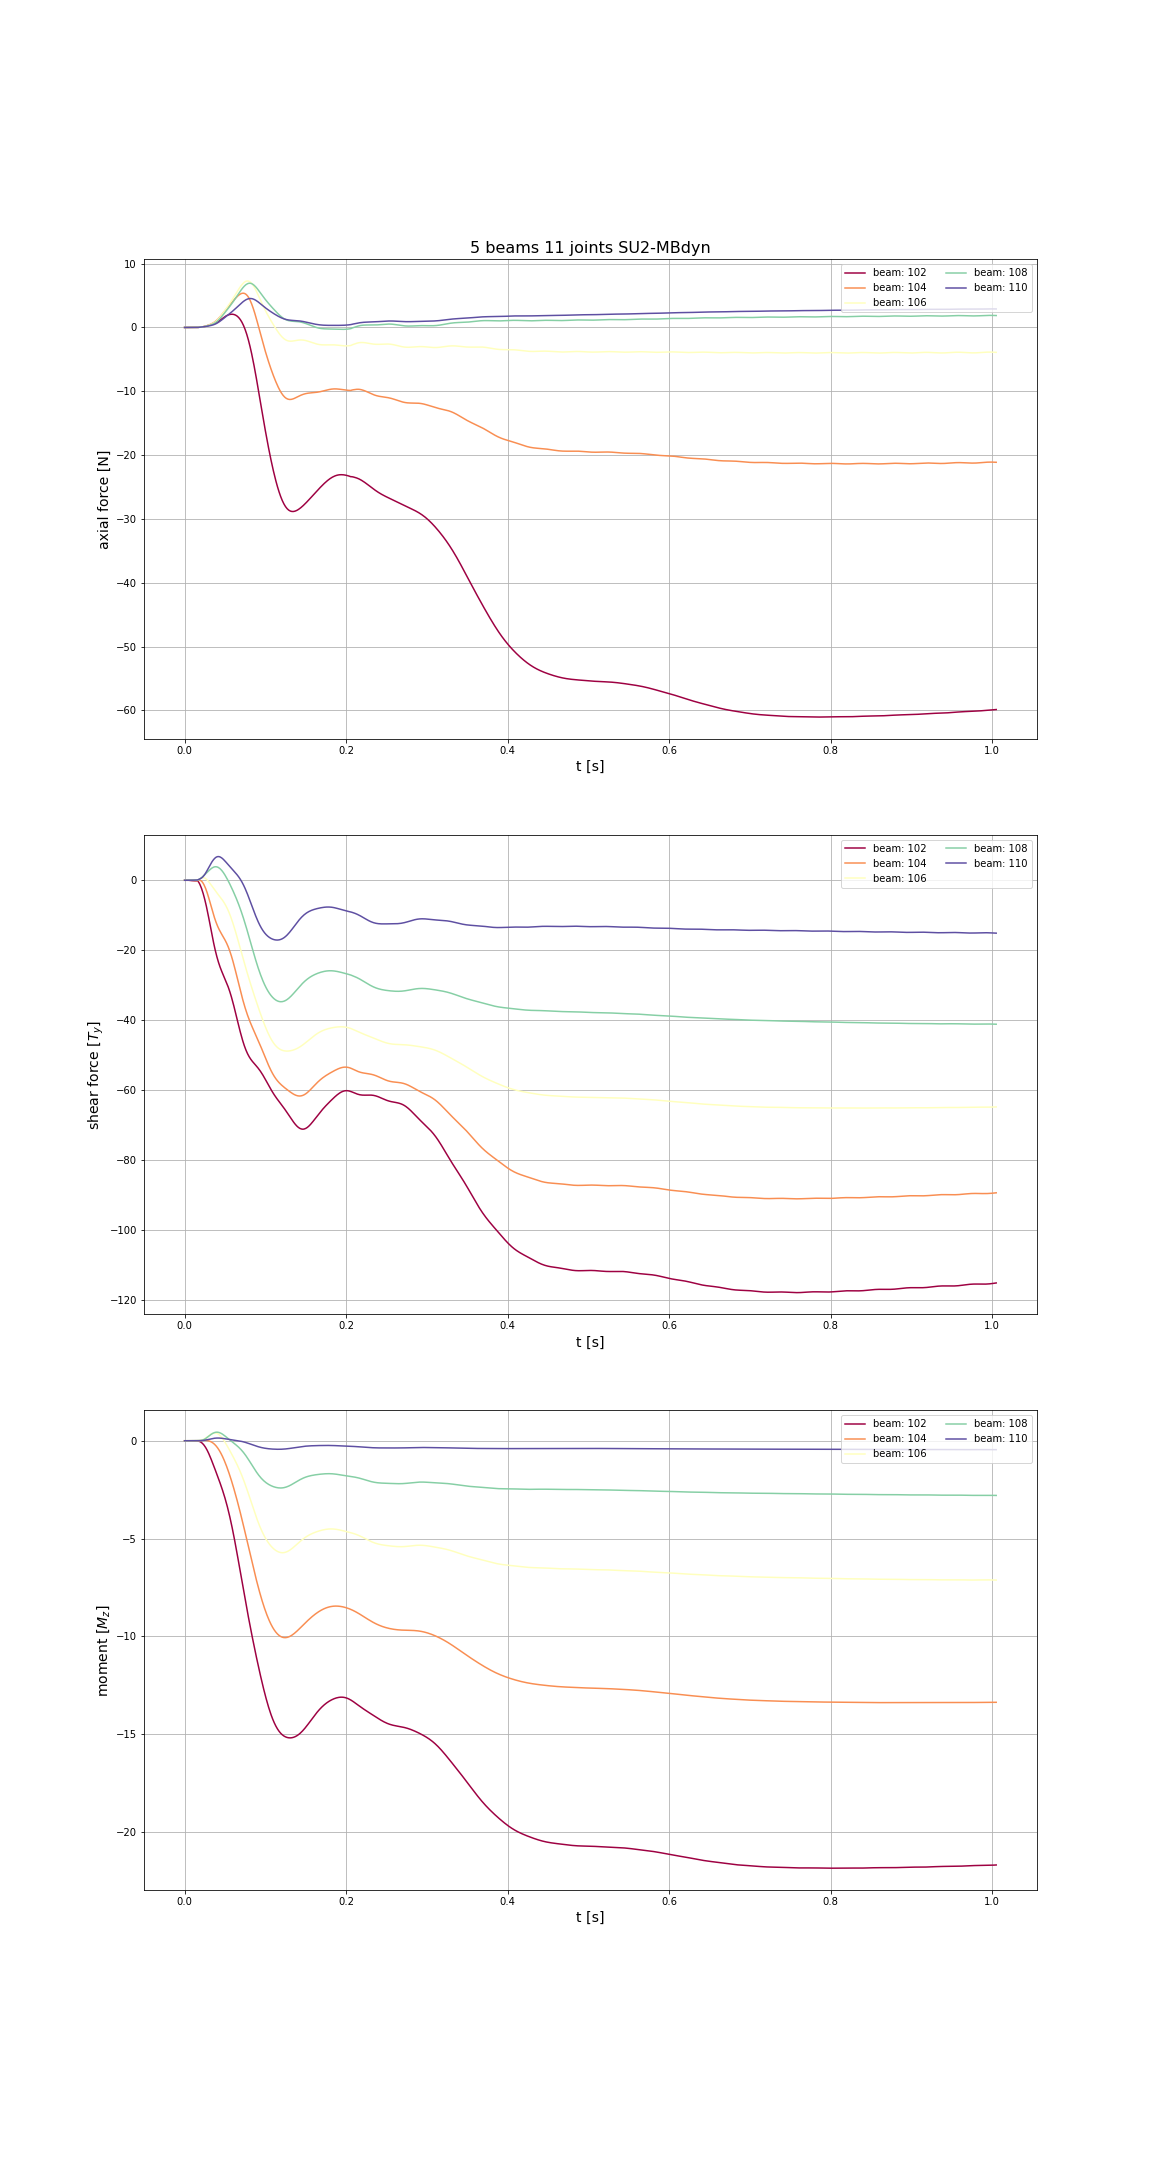
\includegraphics[width=0.92\textwidth, trim=0 230 0 230, clip]{images/comp_flap/vert-flap_SU2-MBDyn_act.png}
	\caption{vertical flap (compressible): MBDyn internal forces}
	\label{fig:comp_mbd_internal}
\end{figure}


\newpage


\section{Square cylinder Benchmark}
\label{sec:sq-cyl-bench}




\subsection{Problem Description}

\cite{ramm1998fluid} art originale.


\subsubsection{Fluid domain}


\subsubsection{Solid domain}


\subsubsection{Coupling parameters}


\subsubsection{Results}

\cite{ramm1998fluid} art originale.
\cite{ramm1998fluid} art originale.
\cite{walhorn2002space}
\cite{matthies2003partitioned}
\cite{dettmer2006computational}
\cite{olivier2009fluid}
\cite{wood2010partitioned}
\cite{kassiotis2011nonlinear}
\cite{habchi2013partitioned}
\cite{froehle2014high}






















\section{Turek-Hron FSI2 Benchmark}
\label{sec:FSI2}
\cite{turek2006proposal}
























\section{Turek-Hron FSI1 and FSI3 Benchmark}
\label{sec:FSI1-FSI3}

The other benchmark proposed in \cite{turek2006proposal}



\begin{table}[!htb]
	\begin{center}
		\begin{tabular}{ l c | r } 
			parameter & & value   \\ 
			\hline
			mass number  & $M$ & $1$     \\
			reduced velocity & $U_R$ & $9.13\cdot 10^{-5}$  \\
			Cauchy number  & $C_Y$ & $2.5\cdot 10^{-5}$  \\			
		\end{tabular}
	\end{center}
	\caption{FSI3: adimensional numbers}
	\label{fsi3:ex1-adim}
\end{table}























\section{Sensitivity analysis of FSI1-FSI3 Benchmarks}
\label{sec:FSI3-sensitivity}

\subsection{FSI1 sensitivity Analysis (Re=20)}


\subsection{FSI3 sensitivity Analysis (Re=200)}


\subsection{Sensitivity Analysis at (Re=1000)}

\subsection{Conclusions}
